\documentclass[11pt, a4paper]{article}

\usepackage{graphicx}
\usepackage[a4paper,top=3cm,bottom=2cm,left=2cm,right=2cm,marginparwidth=1.75cm]{geometry}
\usepackage[english]{babel}
\usepackage[utf8x]{inputenc}
\usepackage{subfig}
\usepackage{float}
\usepackage{amsmath}
\usepackage{amssymb}
\usepackage{mhchem}
\usepackage{hyperref}
\usepackage{tikz}
\usepackage{cancel}

\graphicspath{ {./images} }
\newcommand*{\qed}{\hfill\ensuremath{\quad\square}}%
\newcommand*{\rad}{\ensuremath{\,\text{rad}}}
\newcommand*{\R}{\ensuremath{\mathbb{R}}}
\newcommand*{\C}{\ensuremath{\mathbb{C}}}
\renewcommand*{\Re}{\operatorname{Re}}
\renewcommand*{\Im}{\operatorname{Im}}
\renewcommand*{\epsilon}{\varepsilon}
\renewcommand*{\phi}{\varphi}

\makeatletter
\renewcommand*\env@matrix[1][*\c@MaxMatrixCols c]{%
  \hskip -\arraycolsep
  \let\@ifnextchar\new@ifnextchar
  \array{#1}}
\makeatother

\newtheorem{theorem}{Theorem}

%------------------------------------------------
%Templates for images and figures
% \begin{figure}[h]
%   \centering
%   \subfloat[caption 1]{{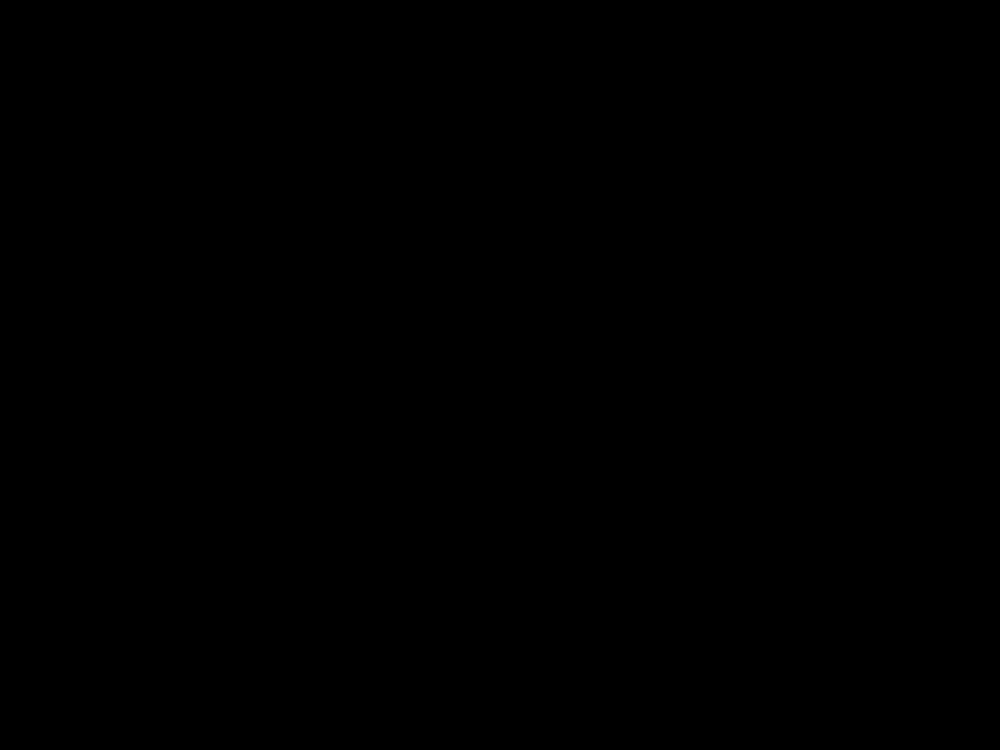
\includegraphics[width=30mm]{images/placeholder.png}}}%
%   \qquad
%   \subfloat[caption 2]{{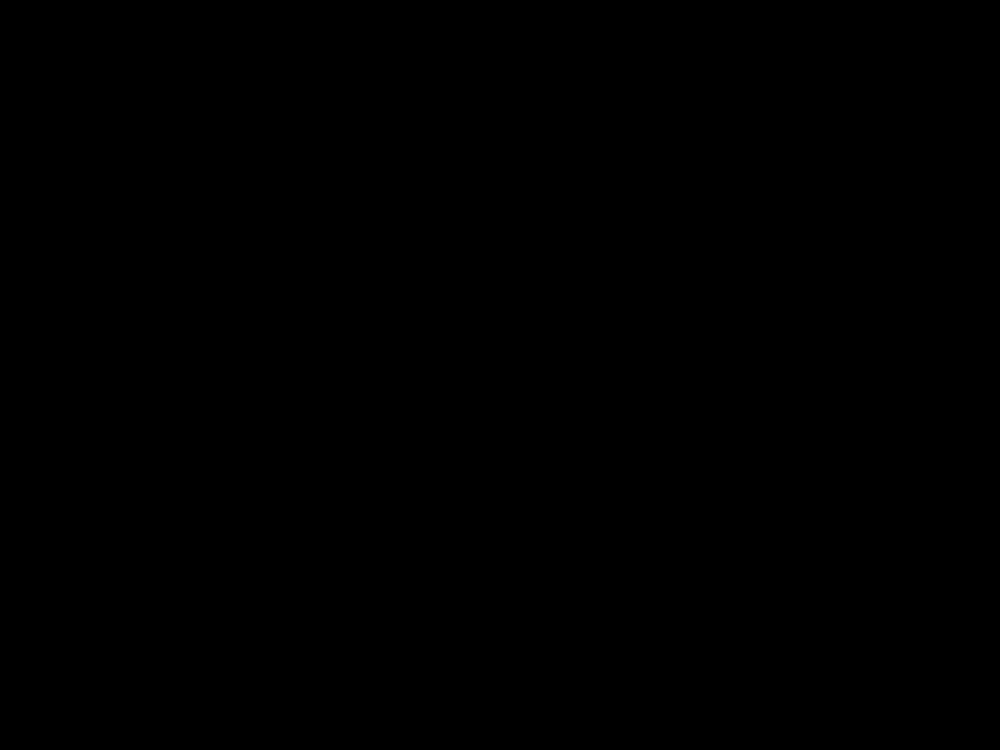
\includegraphics[width=30mm]{images/placeholder.png}}}%
%   \caption{Description}
% \end{figure}

% \begin{figure}[h]
%   \centerline{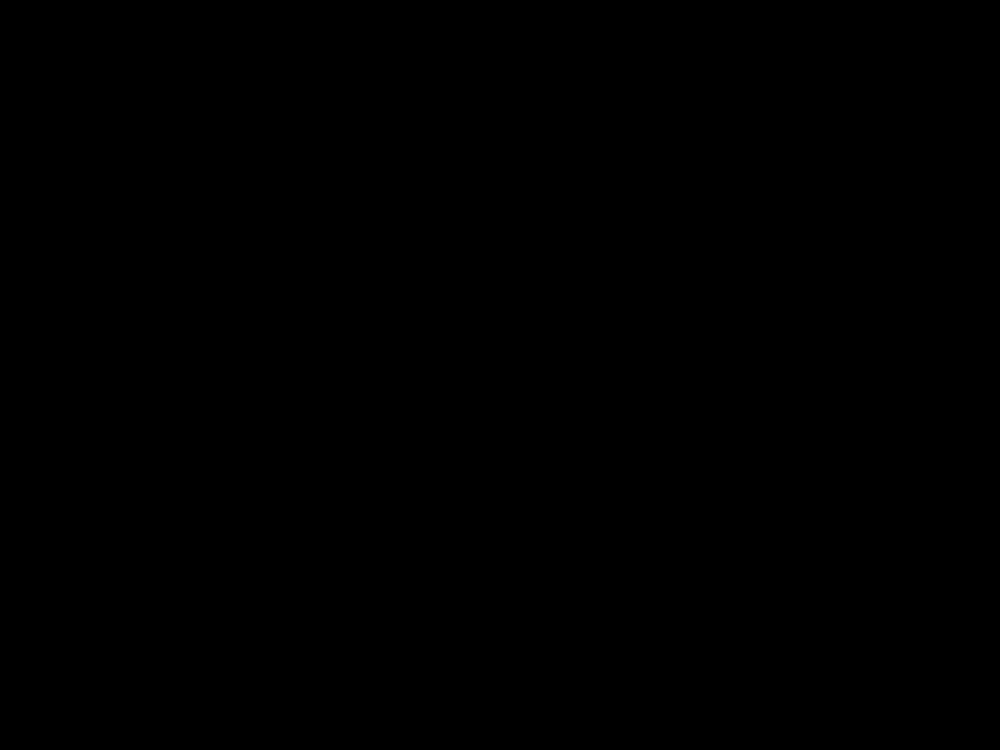
\includegraphics[width=50mm]{images/placeholder.png}}
%   \caption{Description}
% \end{figure}

%Template for a simple table 
%\begin{table}[h]
%   \caption{Description} %title of the table
%   \centering % centering table
%   \begin{tabular}{l rr} % creating three columns
%     \hline\hline %inserting double-line
%     & & \\ [0.5ex] % Insert half line vertical spacing
%     \hline % inserts single-line
%     & & \\ 
%     & & \\
%     & & \\
%     & & \\
%   \hline % inserts single-line
%   \end{tabular}
%   \label{tab:hresult}
% \end{table}
%-----------------------------------------------

\begin{document}

\section{Precision, accuracy and resolution}


\subsection{Level 1: Defining precision, accuracy and resolution}
Systems can be precise but not accurate or accurate but not precise. Precision and accuracy are not the same. To properly quantify precision and accuracy we need to properly define them first.
\begin{itemize}
  \item Precision/Repeatability is defined as tge range of positions measured when a system is repeaditly commanded to one location under identical conditions (the 95\% symmetric interval.) Higher precision means smaller deviation away from the mean position measured.
  \item Accuracy is the difference between the inteded position of a specific point of interest and the measured position (RMS). Higher accuracy means less deviation away from the intended position.
  \item Resolution is the smallest possible movement of a system. This sometimes also called the step-size of the system.
\end{itemize}
\begin{figure}[h]
  \centerline{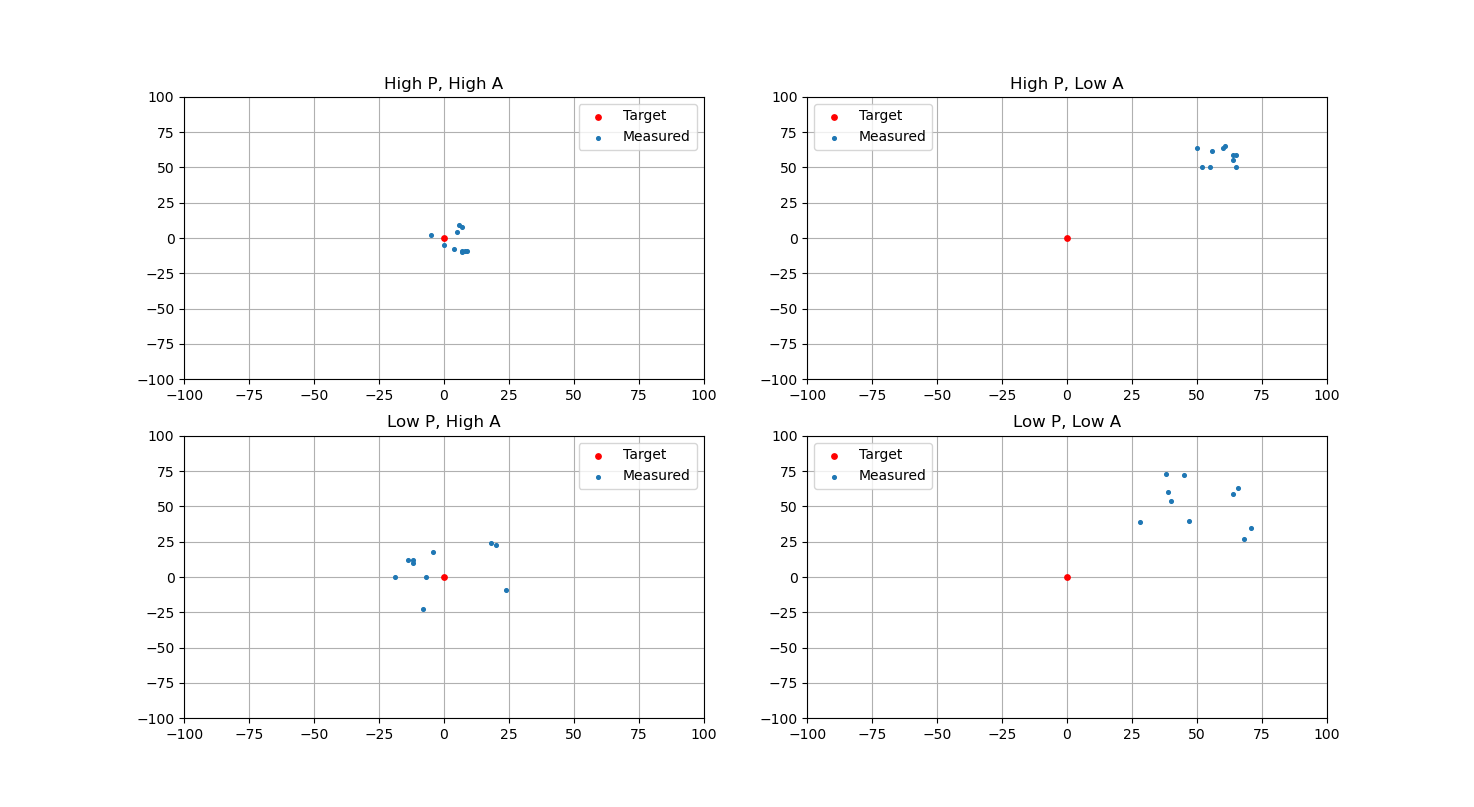
\includegraphics[width=200mm]{images/Accuracy_and_Precision.png}}
  \caption{Visualizing measurements with high accuracy, low accuracy, high precision and low precision.}
\end{figure}
Repeatability can be measured either \underline{unidirectional} or \underline{bi-directional}. Unidirectional approaches the point of interest from one direction and ignores effect from backlash and hysterisis. Bi-directional measures the ability to return to a point from both directions.
The examples of accuracy and precision given in the earlier figure can also be visualized using a normal distribution. A wider curve means lower precision while a narrow curve represents a higher precision. How many standard deviations ($\sigma$) the $x$ target is away from the mean value ($\mu$) represent the accuracy.
\begin{figure}[h]
  \centerline{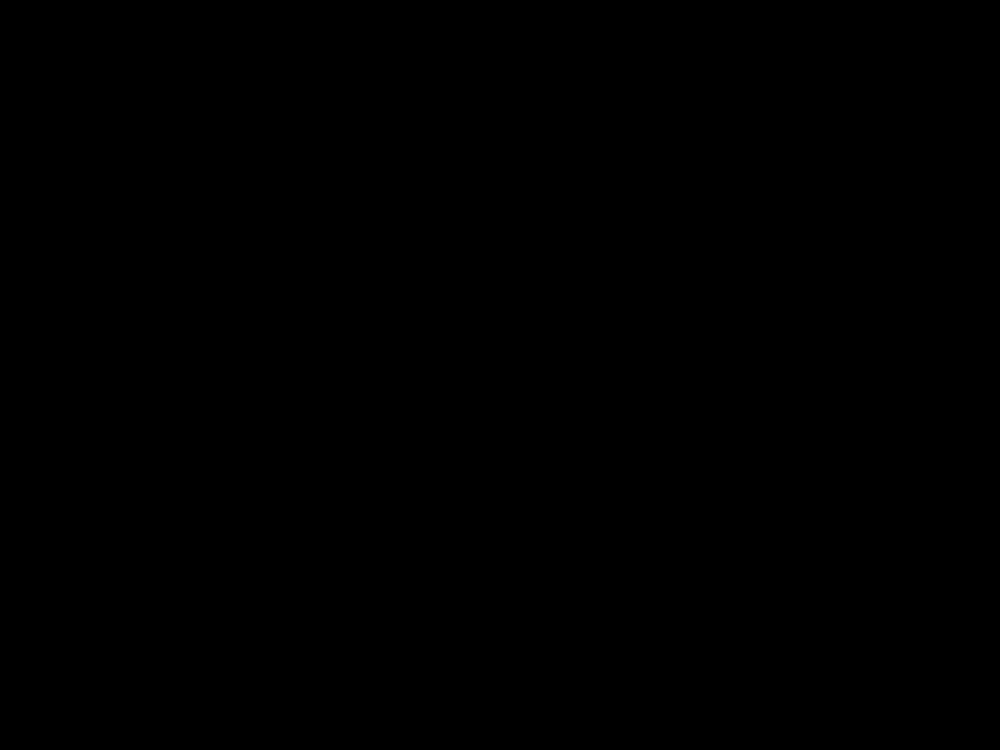
\includegraphics[width=50mm]{images/placeholder.png}}
  \caption{Accuracy and precision represented in a normal distribution.}
\end{figure}
This can all be described numerically using statistics. The mean value of a population or data set can be found using:
\begin{equation}
  \mu = \frac{1}{n}\sum_{i=1}^{n}x_i
\end{equation}
Where $n$ is the amount of samples and $x_i$ the measured values. The standard deviation of some sample of data can then be found using:
\begin{equation}
  \sigma = \sqrt{\frac{1}{n-1}\sum_{i=1}^{n}(x_i - \mu)^2}
\end{equation}
When considering an entire population rather then a sample we replace the $\frac{1}{n-1}$ with $\frac{1}{n}$:
\begin{equation}
  \sigma = \sqrt{\frac{1}{n}\sum_{i=1}^{n}(x_i - \mu)^2}
\end{equation}
To define accuracy we consider how much the data tends to deviate away from the target. This quantity is refered to as the Root Mean Square Error (RMSE).
\begin{equation}
  \text{RMSE} = \sqrt{\frac{1}{n}\sum_{i=1}^{n}(x_i - x_{target})^2}
\end{equation}
To find the precision we look at how large the 95\% confidence interval is using:
\begin{equation}
  \text{CQF} = \pm 1.96\sigma_m
\end{equation}
where $\sigma_m$ can be found using:
\begin{equation}
  \sigma_m = \frac{\sigma}{\sqrt{n}}
\end{equation}


\end{document}